\section{Fremderregter Gleichstromgenerator}
Beim fremderregten Gleichstromgenerator wird die Hauptfelderregung $\Theta_E$ über einen separaten Erregerkreis (Erregerwicklung $F1$-$F2$) eingestellt und kann daher unabhängig vom Laststrom $I_A$ und der Drehzahl $n$ gewählt werden.\\
\subsection{Leerlaufkennlinien}
\begin{figure} [htb]
    \centering
    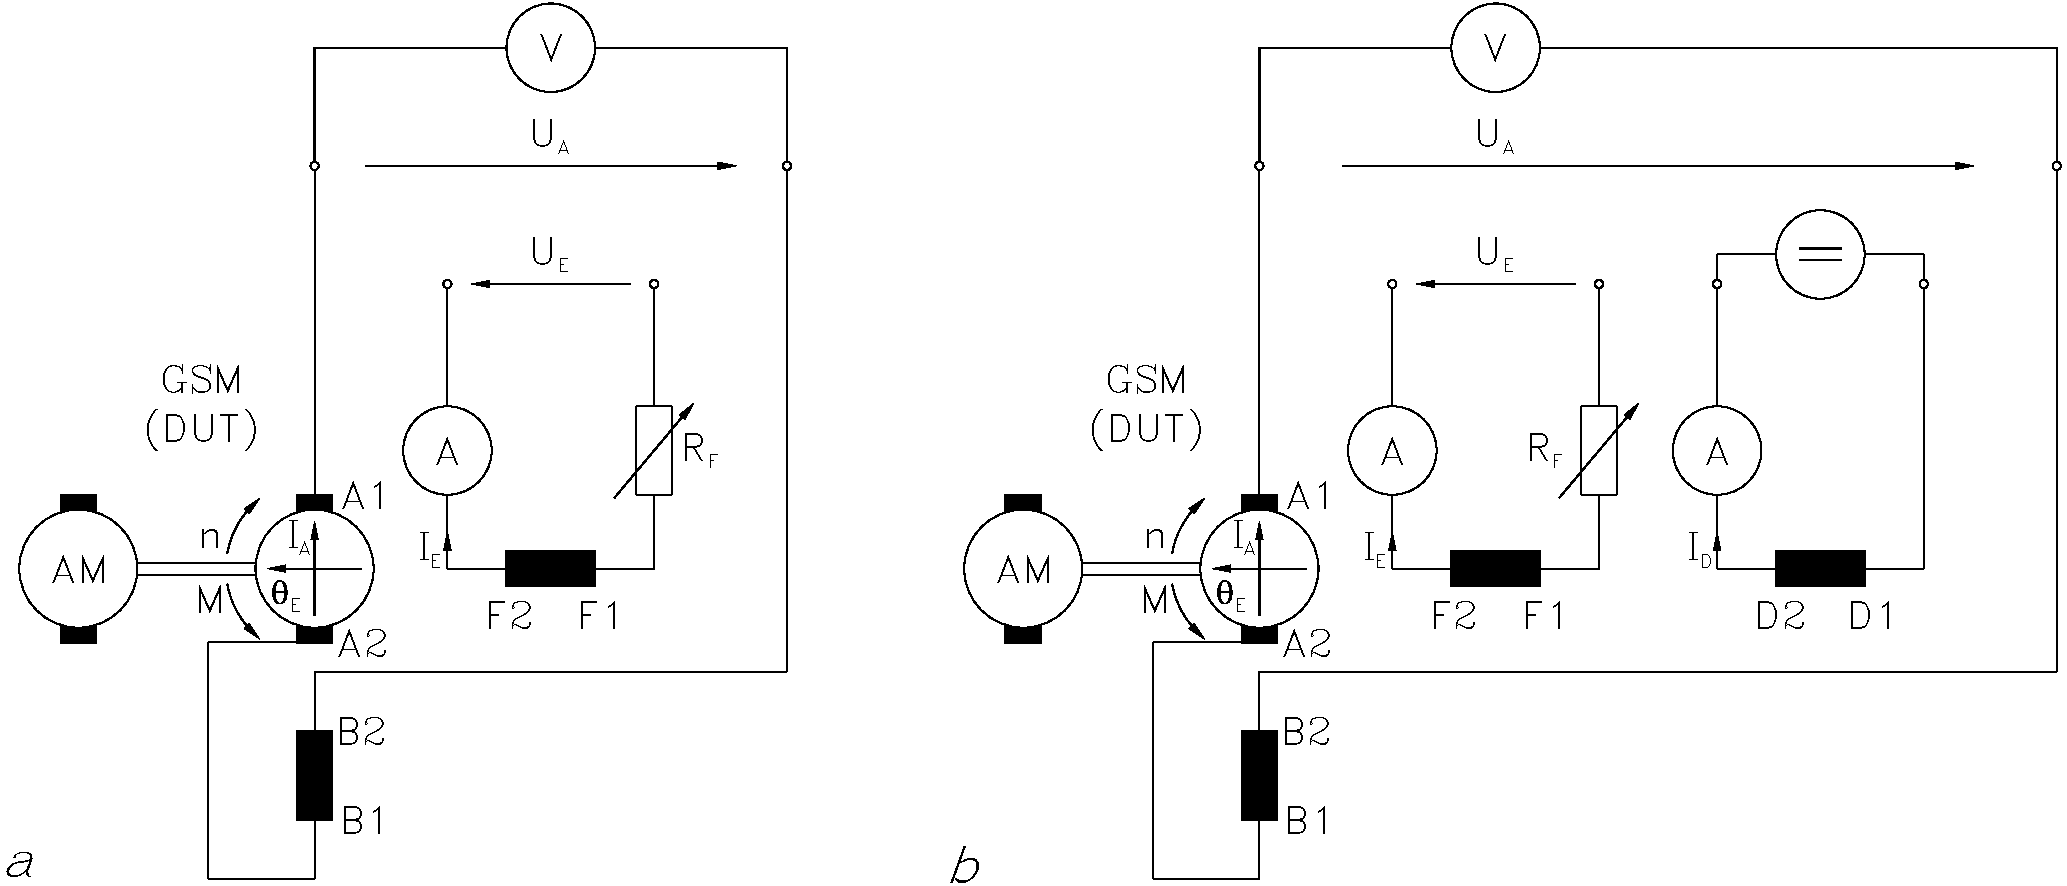
\includegraphics[width=1\textwidth, angle=0]{\currfiledir images/Leerlaufkennlinie_fremd_und_RS}
    \caption{Messschaltungen zur Ermittlung der Leerlaufkennlinie: (a) fremderregter Gleichstromgenerator (GSM), (b) fremderregter Gleichstromgenerator mit fremdbestromter Reihenschlusswicklung ($D1$-$D2$).}
    \label{abb:fremd_LL_Messschaltung}
\end{figure}
\noindent Die Leerlaufkennlinie stellt die innere Spannung in Abhängigkeit der Durchflutung bzw. des Erregerstromes bei konstanter Drehzahl dar.\\
Für deren Bestimmung wird daher eine konstante Drehzahl ($n=n_N$) über die Antriebsmaschine ($AM$) eingeprägt und (bei offenen Klemmen, $I_A = 0$) die innere Spannung $U_A=U_i$ gemessen.\\
Da die Maschine zwei Erregerwicklungen besitzt, wurden zwei Messungen durchgeführt.\\
Bei der ersten Messung wurde die Maschine nur fremderregt betrieben, d.h. die Erregerwicklung $F1$-$F2$ wurde über die Hausbatterie des Labors mit Nennspannung $U_E=U_{E,N}$ versorgt und über einen Vorwiderstand $R_F$ der Erregerstrom $I_E$ variiert. Im zweiten Durchgang wurde die Reihenschlusswicklung ($D1$-$D2$) mit konstanten \SI{40}{\ampere} bestromt und der Strom durch die fremderregte Erregerwicklung wieder variiert. D.h. die Reihenschlusswicklung liefert ihrerseits einen konstanten Erregerbeitrag von $\approx\SI{30}{\percent}$ der Nennerregung $\Theta_{E,N}$.\\
Damit ergeben sich eine Leerlaufkennlinie für die (rein) fremderregte GSM (\SI{0}{}-\SI{50}{\percent} Flussniveau, siehe Abb.\;\ref{abb:fremd_LL_BL_Innen}) und für die Kombination der beiden Erregerwicklungen (\SI{0}{}-\SI{80}{\percent} Flussniveau, siehe Abb.\;\ref{abb:fremd_reihen_LL}).


\subsection{Belastungskennlinie}
\begin{figure} [htb]
    \centering
    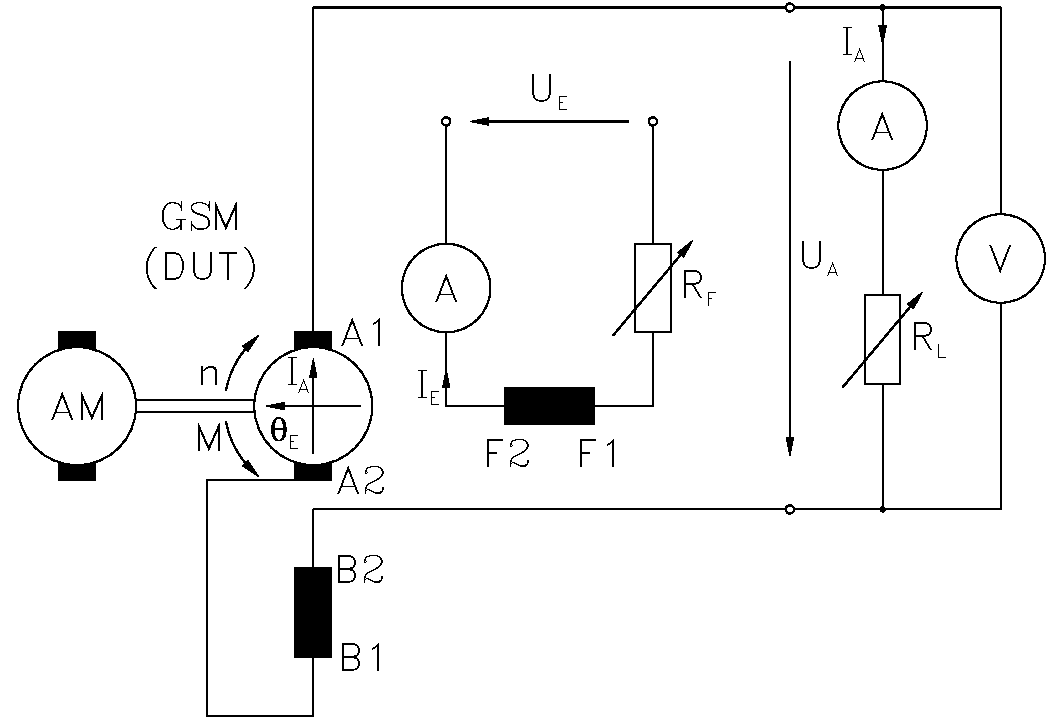
\includegraphics[width=0.55\textwidth, angle=0]{\currfiledir images/Belastungskennlinie_fremderregt}
    \caption{Messschaltung zur Ermittlung der Belastungskennlinie (äußeren Kennlinie und der Regulierkennlinie) des fremderregten Gleichstromgenerators (GSM).}
    \label{abb:fremd_BKL_Messschaltung}
\end{figure}
Nun wurde die Schaltung über einen Leistungswiderstand $R_L$ belastet. Die Drehzahl bleibt dabei unverändert bei $n=n_N$, während Nennerregung $I_E=\SI{1.75}{\ampere}$ gewählt wurde. Der Belastungswiderstand wurde so eingestellt, dass der Ankerstrom bei \SI{50}{\ampere} und die Klemmenspannung bei \SI{200}{\volt} zu liegen kommen. Nun wurde der Erregerstrom stufenweise reduziert und der Ankerstrom über den Belastungswiderstand konstant gehalten. Die resultierende Kennlinie ist in Abbildung \ref{tab:Fremderregt_Belastung} zu sehen. Diese liegt aufgrund der Flussminderung durch den Ankerstrom und den Spannungsabfall am Ankerwiderstand $R_A$ unterhalb der Leerlaufkennlinie.
\subsection{Äußere Kennlinie}
Bei der Äußeren Kennlinie wird die Ankerspannung in Abhängigkeit des Ankerstroms bei konstanter Drehzahl $n=n_N$ aufgenommen. Zu Beginn wird der Erregerstrom $I_E$ so gewählt, dass sich eine Klemmenspannung von \SI{200}{\volt} und ein Ankerstrom von \SI{50}{\ampere} einstellt. Danach wurde die Klemmenspannung gemssen während der Belastungswiderstand $R_L$ schrittweise erhöht wurde, wodurch der Ankerstrom sinkt. Die Gleichung
\begin{equation*}
    U_A=U_i - R_A I_A
\end{equation*}
beschreibt das vorliegende Verhalten in Abbildung \ref{abb:fremd_aussen_regulier} sehr gut. Die GSM verhält sich also wie eine ideale Spannungsquelle mit Innenwiderstand. Für höhere Ströme bzw. eine höhere Erregung wird das lineare Verhalten durch die enstehende Ankerrückwirkung durch die Sättigung des Eisens verzerrt.
\subsection{Innere Kennlinie}
Die Innere Kennlinie lässt sich aus der Belastungskennlinie berechnen. Ein Blick auf die Messschaltung \ref{abb:fremd_BKL_Messschaltung} liefert folgende Gleichung:
\begin{equation*}
    U_i=U_A + R_A I_A
\end{equation*}
Der Wert für den Ankerwiderstand $R_A$ kann den Maschinendaten entnommen werden und entspricht \SI{0.78}{\ohm}. Die so entstandene Kennlinie ist in Abbildung \ref{abb:fremd_LL_BL_Innen} dargestellt.
\subsection{Regulierkennlinie}
Bei der Regulierkennlinie wird der Erregerstrom $I_E$ als Funktion des Ankerstroms $I_A$ dargestellt. Dabei wird die Ankerspannung konstant auf \SI{200}{\volt} gehalten und die Drehzahl wieder auf $n=n_N$ eingestellt.\\
Der Belastungsstrom wurd durch den Lastwiderstand $R_L$ variiert und im Anschluss wird der Erregerstrom über den Vorwiderstand manuell geregelt, sodass sich wieder eine Klemmenspannung von \SI{200}{\volt} ergibt. In Abbildung \ref{abb:fremd_aussen_regulier} ist der Verlauf zu sehen. Die Beziehung zwischen dem Felderregerstrom $I_E$ und dem Ankerstrom $I_A$ ist nahezu linear. Das liegt daran, dass bei steigender Belastung die induzierte Spannung und somit der magnetische Fluss steigen müssen, um die Spannung $U_A$ konstant halten zu können. Bei einer höheren Belastung als Nennstrom $I_{A,N}$ steigt der benötigte Erregerstrom $I_E$ überproportional an, da nun das Eisen zu sättigen beginnt. Die Folge ist eine Kennlinie die bis ungefähr $I_A = I_{A,N}$ linear verläuft.
\input{\currfiledir Fremd_und_Reihen_LL}
\input{\currfiledir Fremderregt_LL_BL_Innen}
\input{\currfiledir Fremderregt_Aussen_Regulier}
%\input{\currfiledir schaltung}